% Сохраняем двухстраничное оглавление и архивные номера страниц теории.
\addtocontents{toc}{\protect\newpage}
\section{ПРАКТИЧЕСКАЯ ЧАСТЬ}
% Численные результаты из analysis.py
\newcommand{\OverviewStep}{10}
\newcommand{\FineStep}{0{,}2}
\newcommand{\PeakEarly}{0{,}00}
\newcommand{\PeakLate}{3{,}40}
\newcommand{\PeakDelay}{3{,}40}
\newcommand{\DelayLower}{3{,}38}
\newcommand{\DelayUpper}{3{,}42}
\newcommand{\GroupIndex}{1{,}50}
\newcommand{\LengthMeters}{680}
\newcommand{\LengthKm}{0{,}680}
\newcommand{\LengthLower}{676}
\newcommand{\LengthUpper}{684}
\newcommand{\ReferenceIndex}{1{,}4682}
\newcommand{\ReferenceLength}{694}
\newcommand{\BackgroundLimit}{-0{,}60}
\newcommand{\WindowStart}{-1{,}5}
\newcommand{\WindowEnd}{8{,}0}
\newcommand{\AreaRatio}{0{,}853}
\newcommand{\PathLoss}{0{,}69}
\newcommand{\EffectiveLoss}{1{,}02}
\newcommand{\PulseRows}{%
  Короткое & 19 & \(-1{,}10502\) & 0,660 & 4,837 \\
  Длинное & 5 & \(-1{,}10618\) & 0,715 & 4,126 \\
}
\newcommand{\SensitivityRows}{%
  5,0 & Среднее & \(-0{,}60\) & 0,683 \\
  6,0 & Среднее & \(-0{,}60\) & 0,688 \\
  8,0 & Среднее & \(-0{,}60\) & 0,691 \\
  8,0 & Медиана & \(-0{,}60\) & 0,701 \\
  8,0 & Среднее & \(-1{,}00\) & 0,692 \\
}


\subsection{Схема измерения}

Первый разветвитель делит импульс лазера между двумя плечами.
Одно плечо короткое, в другое включена катушка волокна.
Второй разветвитель направляет обе копии импульса на один
фотоприёмник. Копия, прошедшая через катушку, приходит позже.

\begin{figure}[H]
\centering
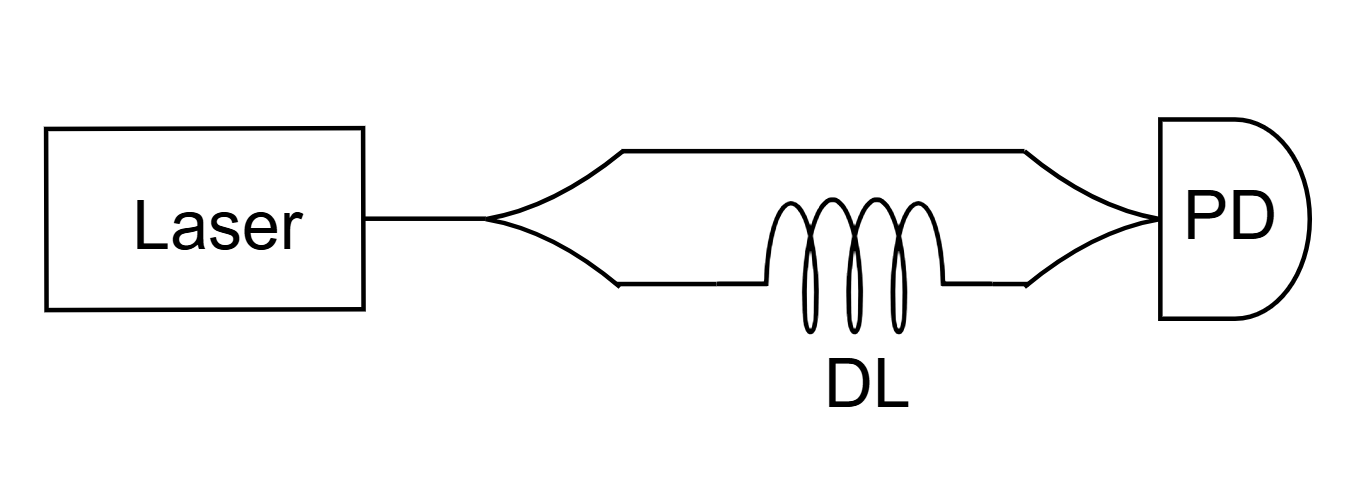
\includegraphics[width=0.66\linewidth]{Setup.png}
\caption{Схема установки. DL~--- катушка волокна, PD~--- фотоприёмник}
\end{figure}

На осциллографе LeCroy оба импульса записали на общей шкале с
шагом \(\OverviewStep\)~нс (файл \texttt{C2300000.txt}).
Затем записали каждый импульс с шагом \(\FineStep\)~нс.
По порядку регистрации файл \texttt{C2300001.txt} соответствует
короткому плечу, \texttt{C2300002.txt}~--- плечу с катушкой.

\subsection{Длина линии}

На общей осциллограмме пики разделены на \(\PeakDelay\)~мкс
(рисунок~\ref{fig:delay}). Это задержка, которую вносит
длинное плечо. Длину соединительных отрезков считаем малой
по сравнению с длиной катушки. При групповом показателе
преломления \(\GroupIndex\) свет проходит около \(200\)~м за
микросекунду~\cite{agrawal}. Получаем
\[
  L \approx \frac{c}{\GroupIndex}\cdot\PeakDelay~\text{мкс}
    \approx \LengthMeters~\text{м}.
\]

\begin{figure}[H]
\centering
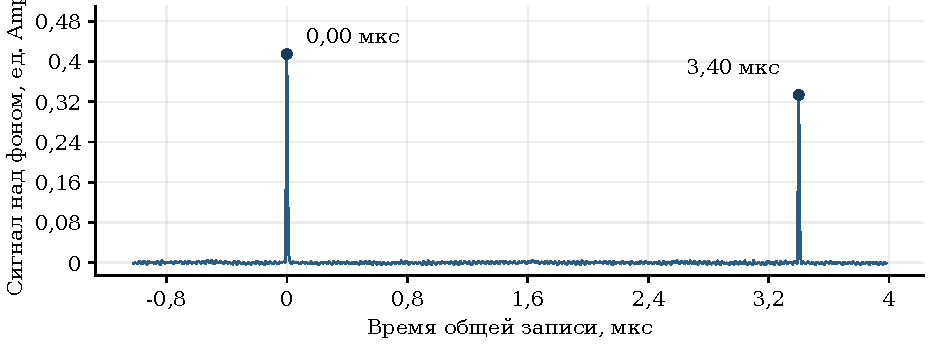
\includegraphics[width=0.94\linewidth]{figures/delay.pdf}
\caption{Два импульса на общей осциллограмме. Маркеры показывают
время прихода по максимальному отсчёту каждого импульса}
\label{fig:delay}
\end{figure}

\subsection{Затухание}

Из каждой записи вычли среднее по участку до подъёма.
Фронты совместили по полувысоте, сохранив масштаб амплитуд.
От точки совмещения отсчитали окно от \(\WindowStart\)
до \(\WindowEnd\)~нс. В окно входят основной импульс и часть
хвоста, видимая на обеих записях.

\begin{figure}[H]
\centering
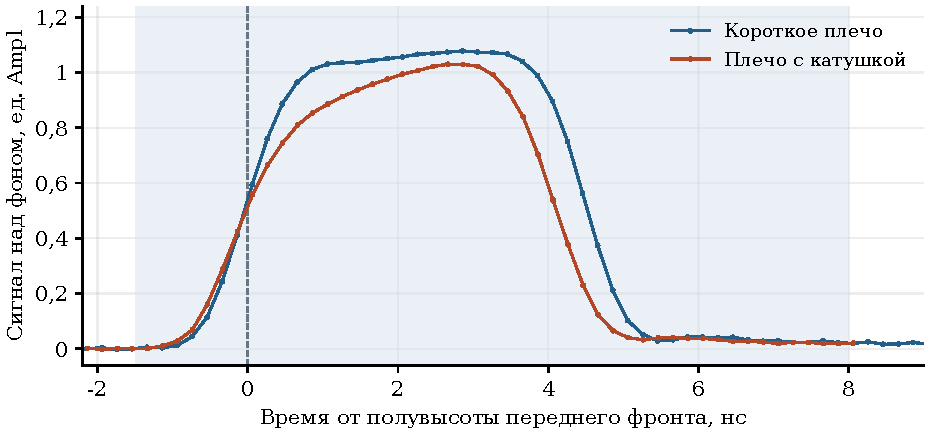
\includegraphics[width=0.94\linewidth]{figures/pulses.pdf}
\caption{Импульсы на одной амплитудной шкале после вычитания фона.
Заливка показывает окно, в котором рассчитаны площади}
\label{fig:pulses}
\end{figure}

Фотоприёмник преобразует оптическую мощность в электрический сигнал.
Площадь учитывает и высоту, и длительность импульса, поэтому
отношение площадей даёт оценку потери энергии в выбранном окне.

\begin{samepage}
По правилу трапеций получены площади \(\ShortArea\) для короткого
плеча и \(\LongArea\) для плеча с катушкой в ед.~шкалы\(\cdot\)нс.
Затухание между плечами составило
\[
   10\lg\frac{\ShortArea}{\LongArea}=\PathLoss~\text{дБ}.
\]
\end{samepage}
При изменении границы окна и способа оценки фона получалось
от \(\LossLower\) до \(\LossUpper\)~дБ.
В пересчёте на длину катушки получаем \(\EffectiveLoss\)~дБ/км.
В измерение входят потери катушки и её соединений, а также
разница в пропускании портов разветвителей.

\subsection{Контроль входа осциллографа}

На RIGOL сравнили импульсы без катушки при входах \(50\)~Ом
и \(1\)~МОм. При \(1\)~МОм примерно через \(10\)~нс после фронта
виден отрицательный выброс. При \(50\)~Ом отклонение на этом
участке меньше (рисунок~\ref{fig:load}).

\begin{figure}[H]
\centering
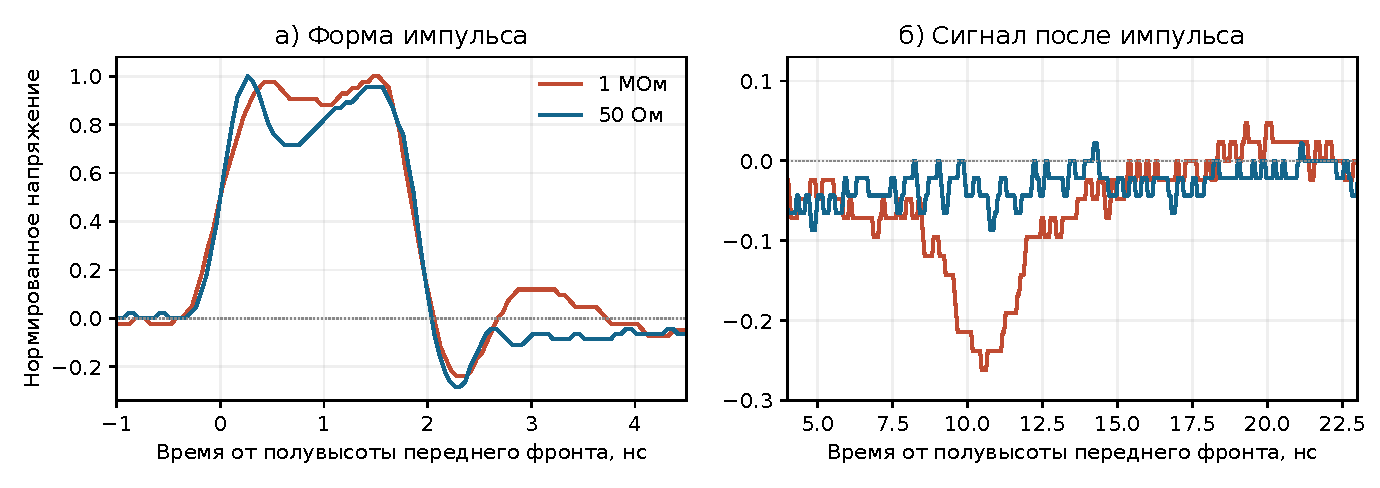
\includegraphics[width=0.94\linewidth]{figures/detector_load.pdf}
\caption{Контрольная запись без катушки. Амплитуды приведены
к максимуму каждой кривой для сравнения формы импульсов}
\label{fig:load}
\end{figure}

\section*{ЗАКЛЮЧЕНИЕ}
\phantomsection
\addcontentsline{toc}{section}{ЗАКЛЮЧЕНИЕ}

Задержка \(\PeakDelay\)~мкс соответствует длине волокна
около \(\LengthMeters\)~м при групповом показателе преломления
\(\GroupIndex\). В плече с катушкой сигнал ослаб на
\(\PathLoss\)~дБ относительно короткого плеча, что даёт
\(\EffectiveLoss\)~дБ/км в пересчёте на длину волокна.
